
\chapter{背景知识}\label{sec:req}

本研究的主要内容是基于Zynq SoC平台实现高性能的深度学习框架,因此涉及到三个领域的基本内容:深度学习与神经网络,系统芯片(System-on-Chip,简称SoC),以及可编程逻辑门阵列(Field Programmable Gate Array,简称FPGA)和高层次综合(High-Level Synthesis,简称HLS)。本章分别介绍上述三个领域的基本原理,并选择与本研究密切相关的细分方向进行具体分析。

% 基本原理部分
\section{深度学习与神经网络}

深度学习属于机器学习领域的一个新兴分支。
% 简单介绍机器学习的概念:学习历史数据
机器学习是实现人工智能的一种方法,简单而言,机器学习往往从大规模的历史数据中学习规律,进而对新的样本进行分类(classification)和预测(prediction)。传统的机器学习算法需要人工指定学习规则,比如从样本中提取哪类特征(feature)、用哪种统计模型进行训练等等。此类方法虽然直观,但需要大量的工程和领域(domain)相关的知识才能达到不错的效果。面对人类认知范围之外的模型时,往往特征提取和模型训练的效果都不尽如人意,有时甚至完全提取不出合适的特征。

% 简单介绍深度学习的历史背景,引出后续的讨论
深度学习系统的设计是革命性的:特征不再是由专家设计,而是交给通用的算法来自动学习。具体而言,深度学习将特征组织成从低到高的多层堆叠的特征层,使用反向传播算法(Back-propagation,简称BP)提取特征。深度学习与人脑的工作原理密切相关,堆叠连接的特征层本质上是对神经元的模拟。从这个角度看,深度学习与神经网络是密不可分的:深度学习中的特征层和反向传播算法都来自神经网络。本节接下来首先介绍深度学习的基本概念与基本流程,之后介绍神经网络的几种网络层的特性,其中着重介绍卷积神经网络。

\subsection{深度学习}

2015年5月,深度学习领域的三位代表人物Yann LeCun\footnote{Yann LeCun目前为纽约大学教授,Facebook人工智能研究院负责人},Yoshua Bengio\footnote{Yoshua Bengio为加拿大蒙特利尔大学教授}与Geoffrey Hinton\footnote{Geoffrey Hinton为加拿大多伦多大学教授,并且任职与Google}在《自然》杂志发表封面文章《Deep Learning》\supercite{lecun2015deep},介绍深度学习的基本概念与发展现状。
% 表征学习与深度学习
文章将深度学习归纳为表征学习(Representation Learning)\supercite{bengio2013representation}的一类方法。表征学习即学习如何从原始数据中提取出可以用来训练与学习的特征的过程,深度学习在此之上使用多层表征,每层的特征与上层相比更抽象。此外,每一层都获取上层的输出特征作为输入,进行非线性的转换之后输出到下一层。每层的转换方程都有特定的权值,显著的权值可以放大某些输入特征的“影响”,相应地不显著的权值则“隐藏”了无用的输入特征。深度学习应用经过训练之后,得到的权值可以使得每层提取出最合理的特征。由此看出,深度学习几乎不依赖人类的先验知识,给定特征层的结构和训练数据集之后便可以学习到最合适的特征形式。接下来简单介绍深度学习的训练过程。

% 监督学习
所谓训练,即通过历史数据修正深度学习各层中的权值。深度学习的训练有三个基本概念:训练集,损失函数(Loss function)与随机梯度下降(Stochastic Gradient Descendent,简称SGD)。训练集由大规模的输入数据与预期的输出结果组成,比如图像识别应用往往使用标记好类型的图片集作为训练集。训练集的好坏很大程度上决定了训练结果的好坏。损失函数衡量预期结果与当前系统预测结果的区别,衡量了当前训练阶段的成果,给下一步对权值的调整方向以反馈信息。随机梯度下降根据损失函数相对于权值在小范围内的梯度对权值进行调整。训练集、损失函数与随机梯度下降构成了完整的深度学习训练过程。使用训练集并进行训练的深度学习也称之为有监督学习(Supervised Learning)。

\subsection{神经网络}

% 历史
神经网络与深度学习不是一类概念,深度学习是一种机器学习的方法,而神经网络则是从生物神经元的构成和连接启发的一种
计算过程或组织形式。深度学习侧重方法,神经网络偏重结构。深度学习定义了分层的表征学习结构,而神经网络提供了更具体的计算细节。神经网络起源于19世纪60年代的感知器(Perceptron)模型,它抽象了生物的神经元:神经元接受一组信号的输入,通过权值加权、激活函数等等的计算得到结果。神经网络将神经元组织成大规模的网络结构,相同类型的神经元组成神经网络层,提供特殊形式的计算。这种分层的神经网络结构与深度学习不谋而合。

% 反向传播算法
深度学习中提到的随机梯度下降计算利用了反向传播算法。反向传播算法于19世纪80年代左右发明,主要用来推导多层网络结构中每一层的梯度,进而实现随机梯度下降计算。反向传播算法利用复合函数求导的“链式法则”(chain rule),结合网络的分层结构,可以根据网络顶部的输出结果变化反向传播得到每层输入权值的梯度。反向传播算法也因此成为深度学习训练的基础算法。与反向传播相反,前向传播(Forward propagation)是从神经网络的底层逐层计算到顶层输出结果,反向传播用来求梯度,前向传播则用来预测。

% 神经网络的网络层
神经网络有多种网络层,有些网络层由激活函数构成:比如常用的线性整流层(Rectified Linear Unit,简称ReLU,$f(x)=max(x,0)$),tanh层($f(x)=tanh(x)$)、Sigmoid层($f(x)=\frac{1}{1-exp(x)}$)等等;有些网络层主要是计算,比如卷积层(Convolution Layer)等等。卷积层使用一系列矩阵块(也称为卷积核)对输入值进行卷积计算。神经网络根据组成的网络层以及它们的堆叠方式不同而分类为不同的神经网络类型,卷积神经网络(Convolutional Neural Network,简称ConvNet或CNN)是其中最常用的网络结构之一。

% 卷积神经网络
卷积神经网络的设计来源于生物的视网膜工作原理,网络结构主要由卷积层、池化层(pooling layer)和线性整流层构成:卷积层进行卷积计算提取特征(feature map),池化层按照划分好的区域过滤降维,一般求最大值(max pooling)或均值(mean pooling)。卷积神经网络广泛使用于图像识别、视频分析以至于围棋比赛中,并取得了很好的效果。除了卷积神经网络以外,递归神经网络(Reccurrent Neural Network,简称RNN)在需要“记忆”和上下文信息的学习过程中也起到很大作用,比如文本生成和自然语言处理等。
\begin{figure}[!ht]
\centering
	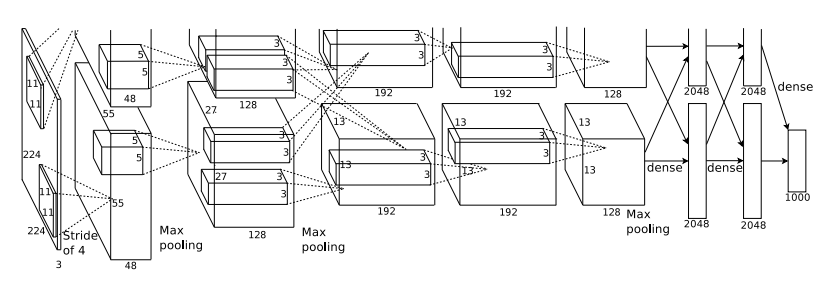
\includegraphics[width=0.8\textwidth]{assets/imgs/imagenet-cnn}
\caption{ImageNet LSVRC-2012比赛中使用的大规模卷积神经网络结构\supercite{krizhevsky2012imagenet}}
\end{figure}

% 总结
综上所述,深度学习是机器学习的全新分支,挑战了传统的机器学习方法论。神经网络通过仿生的神经元与网络设计,具象化了深度学习的特征层与堆叠方式。此外,深度学习涉及到的计算,比如卷积神经网络中的卷积层等等,都十分耗费硬件的计算资源和存储资源。本研究的主要目标即为将传统的、部署于大规模CPU和GPU的深度学习应用,运行于硬件资源和计算能力都十分有限的嵌入式平台上。接下来会对本研究涉及的硬件系统进行详细的介绍。

\section{系统芯片(SoC)}

% SoC的特点
系统芯片(System-on-Chip,简称SoC)是一类集成电路,其上包含了处理器芯片和其他电子系统,以及丰富的外部接口和设备等等。SoC主要被电子工程师用来进行系统开发和验证:SoC的处理器性能足够强大,一般足以运行常见的操作系统;SoC一般也搭载了可编程的FPGA硬件系统,可以非常方便修改硬件系统的设计。因此SoC可以明显缩短电子产品的开发周期。

% SoC的设计流程
SoC的设计分为软件与硬件两部分。软件部分的开发主要涉及偏底层的硬件驱动、数据传输、硬件控制与基于操作系统的高层次软件等等。硬件系统的设计则更加复杂:工程师一方面开发基于FPGA的硬件逻辑,定制系统所要求的特殊功能;另一方面也尽可能基于预定义的、标准的IP核(全称知识产权核,Intellectual Property core)进行基础平台的搭建,提高开发效率。此外,硬件与软件不同,在开发完成之后需要进行各种系统级、行为级的功能验证才能正式完成。正因为SoC开发难度大,目前在开发工具上和平台设计上都有相应的进展,本研究所使用的Xilinx Zynq SoC平台与SDSoC开发工具便是例证。

% SoC与嵌入式系统、研究目标的关系
本研究的目标是将深度学习框架部署于嵌入式平台中。嵌入式设备指的是一类针对特定应用场景开发的硬件设备,这类场景往往对实时性要求高,同时也对功耗与设备尺寸进行限制。SoC作为嵌入式设备的一种实现方式,完整的功能和较低的功耗比兼具,因此非常适合作为本研究的基础开发平台。第二章对本研究使用的Zynq SoC平台与SDSoC开发工具进行详细的介绍。

\section{现场可编程逻辑门阵列(FPGA)}

% FPGA可编程的特性介绍
FPGA(Field Programmable Gate Array,现场可编程逻辑门阵列)是一种特殊的半导体设备,特点在于可以对硬件逻辑进行重复编程。与ASIC(Application-Specific Integrated Circuit,专用集成电路)相比,FPGA比ASIC速度要慢,而且占用更多空间。但ASIC在设计和实现完成之后就不能修改,而FPGA可以不断修改其硬件配置,因此能大大提高硬件开发效率。与CPU相比,FPGA针对特定形式的计算速度更快,而且功耗很低,因此在嵌入式设备和SoC中往往将FPGA视为重要的组成部分。

% FPGA的组成
FPGA的基础组件为CLB(Configurable Logic Block,可配置逻辑块),其中包含LUT(Look-Up Table,查找表)、全加器和触发器(Flip-Flop)等等基本元素。CLB十分灵活,既可以用来实现时序与组合逻辑,也可以用来实现RAM。CLB之间则通过可编程的线路进行连接。FPGA的可编程性主要取决于两个部分:一个是查找表的配置,查找表中包含SRAM与多路选择器,SRAM的值随着硬件逻辑设计不同而不同,进而改变CLB的计算结果;另一个是连接CLB的线路,线路的交叉点也是可以配置进而改变CLB之间互联模式的。除此以外,不同的FPGA版本具有不同的资源配置,比如BRAM(Blocked RAM,块内存)与DSP(Digital Signal Processing,数字信号处理单元)等等在不同的FPGA上具有不同的数量,性能也不尽相同。

% FPGA的工作
传统的FPGA开发使用的是VHDL,Verilog,SystemC等硬件描述语言,这类语言用于表述硬件的寄存器传输级别(Register Transfer Level,简称RTL)的抽象。使用这类语言完成设计并仿真验证之后,便可以使用不同FPGA厂商提供的工具进行FPGA的综合(Sythesis)、实现(Implementation)和比特流生成(Bitstream Generation)。综合把电路的高级抽象转换为底层的逻辑门之间的连接,建立逻辑门网表。实现则是针对具体的FPGA硬件,进行逻辑网表的布局(Placement)、布线(Routing)以及满足资源的限制等等。最后的生成可以编程到FPGA上的比特流,比特流用来配置FPGA上的各类硬件资源。与软件编译相比,FPGA硬件的综合、实现与比特流生成往往需要花费几十分钟到数小时,依FPGA的资源和硬件设计大小而定。

% 总结
综上所述,FPGA具有可重构的硬件逻辑、优异的低功耗以及成熟的开发流程,并且广泛应用在各种计算平台中。FPGA也有其缺点,一方面是开发门槛比较高,没有数字电路基础的软件开发者很难写出性能优秀的FPGA应用;另一方面,FPGA只适用部分的计算过程,涉及到复杂的条件判断、循环等计算过程更适合部署于CPU执行。因此,本研究将FPGA作为硬件加速器,即部署计算量大但逻辑简单的计算过程于FPGA上加速。同时本研究也是用高层次综合工具提高硬件逻辑的开发效率。接下来进一步介绍高层次综合的基本概念和使用方式。

\section{高层次综合}

% 高层次综合的简介,以及优点
高层次综合(High-Level Synthesis,简称HLS)是一种将行为级的、算法级的代码转换为硬件逻辑的过程。高层次综合的输入不再是传统的硬件描述语言,取而代之的是C/C++等高级程序语言。高层次综合使得硬件逻辑开发可以从软件代码开始:传统的开发方式需要等到RTL实现完成之后才能验证,迭代周期很长;而高层次综合工具可以令开发者先实现好软件系统,之后直接把需要在FPGA上加速的代码进行高层次综合即可。通过高层次综合工具,软件工程师可以不用学习RTL级别的描述语言就可以实现硬件逻辑。根据Xilinx的调查显示,基于高层次综合的设计开发方法与传统方法相比时间加快4倍,结果质量提高0.7到1.2倍。

% 高层次综合的基本流程
一般的高层次综合流程包含如下几步:控制流和数据流图(Control Data Flow Graph)分析,资源分配(Resource Allocation),调度(Scheduling),绑定(Binding)等等。高层次综合的流程本质上是求解在资源和时间的约束下,能达到最优的资源分配和调度策略。这种最优解往往依赖启发式的算法,因此高层次综合工具分析的结果往往比较保守,在资源配置和调度上不一定能取得最佳的结果,因此需要通过开发者手动指定生成硬件的选项。比如指定某一运算需要使用DSP实现,某一循环需要流水线化等等。

% 总结
综上,高层次综合工具提供了一种生产力更高的开发FPGA应用的方式,为了取得更高的性能也需要开发者对应用进行分析、手动生成限制条件。本研究使用的SDSoC工具中整合了Xilinx Vivado HLS工具,在后续的硬件加速器的设计中主要用它进行硬件逻辑的实现和优化。
